% ACL-style report. Compile with the official ACL template (acl.sty, acl_natbib.bst), for example in
% Overleaf: upload this file, refs.bib and the four PNG files from ../figs/.
% NOT YET COMPILED: no LaTeX installation was available where this was written.
\documentclass[11pt]{article}
\usepackage[preprint]{acl}
\usepackage{times}
\usepackage{latexsym}
\usepackage[T1]{fontenc}
\usepackage[utf8]{inputenc}
\usepackage{graphicx}
\usepackage{booktabs}
\usepackage{amsmath}
\graphicspath{{../figs/}{figs/}{./}}

\title{Decodable, Misstated and Ignored:\\Do LLM Agents Know Which Actions Cannot Be Undone?}

\author{Author One \and Author Two \and Author Three \\
  Department, University \\
  \texttt{email@domain}}

\begin{document}
\maketitle

\begin{abstract}
AI agents now take actions that cannot be undone. We measure whether two open-weight
instruction-tuned models (Qwen2.5-7B and Mistral-7B) represent the reversibility of an action,
state it when asked, and act on it. The testbed is a simulated file, email and wallet sandbox
built around minimal pairs, in which the same tool call is reversible or irreversible depending
on one line of the state, plus ScienceWorld actions labelled by search (2,710 labelled pairs).
A linear probe on hidden states separates reversible from irreversible actions with balanced
accuracy 0.92 and 0.89, and 0.91 and 0.85 on minimal pairs where a bag-of-words baseline reaches
0.71. The same models answer a direct question about reversibility with 40\% and 42\% accuracy,
and their answers barely agree with the probe ($\kappa \leq 0.15$). As agents on 60 paired tasks,
both take the irreversible action in 95\% of cases and are no more careful than in the reversible
version (sensitivity $+0.02$ and $-0.02$); an explicit instruction does not change this for Qwen.
Steering Qwen along the probe direction changes behaviour in a graded way that a random direction
does not, but in the opposite direction to the hypothesis, and it never makes the agent more
careful in the irreversible version than in the reversible one. The probes also fail to transfer across environments and across tool families.
Reversibility is decodable, but we find no evidence that the decodable signal is what the models
say or use.
\end{abstract}

\section{Introduction}

Agents built on large language models run commands, edit files, send messages and move money.
Some of these actions can be undone and some cannot. A careful person slows down before the
second kind: they check, make a copy or ask. This paper measures whether open-weight LLM agents
do the same, and separates three things that are easy to conflate:

\begin{enumerate}
\item \textbf{Representation.} Can the reversibility of a proposed action be read from the
model's hidden state with a linear probe (RQ1)?
\item \textbf{Statement.} When asked directly, does the model say whether the action can be
undone, and does that answer agree with the probe (RQ2)?
\item \textbf{Behaviour.} When acting, is the agent more careful before an irreversible action
than before the same action in a state where it is reversible (RQ3)?
\end{enumerate}

We add a causal test (RQ4): if the hidden state is pushed along the probe's ``irreversible''
direction during a task, does the agent become more careful?

Reversibility has been studied in reinforcement learning \citep{grinsztajn2021turning,
krakovna2018relative,turner2020aup}, and agent safety benchmarks test risky actions in general
\citep{ruan2024toolemu,yin2024safeagentbench}. \citet{tang2025riskknowledge} show that LM agents
can fail to act on risk knowledge they can state. We are not aware of published work that tests
whether LLM agents internally distinguish reversible from irreversible actions and whether that
distinction reaches action selection.

The central design element is the \emph{minimal pair}: the same tool call, character for
character, whose reversibility is set by one line of the state. A probe or a model that only
reacts to the word ``delete'' cannot solve a minimal pair.

Our findings, for both models:
\begin{itemize}
\item Reversibility is linearly decodable from the upper-middle layers, well above lexical
baselines on minimal pairs. The decodable signal is specific to a tool and its policy; it does
not transfer across environments or to a held-out tool family.
\item Stated answers are poor and nearly unrelated to the probe.
\item Behaviour does not depend on reversibility, with or without an instruction to be careful.
\item Steering along the probe direction is causally effective but does not produce caution.
\end{itemize}
We release the sandbox, the 2,710 labelled pairs, the 60 paired tasks and all logs.

\section{Related Work}

\paragraph{Reversibility and side effects.} \citet{grinsztajn2021turning} learn reversibility
from experience and use it for safer exploration. \citet{krakovna2018relative} and
\citet{turner2020aup} penalise side effects through reachability and attainable utility. These
methods train agents; we measure what a pretrained language model already encodes.

\paragraph{Probing.} Linear probes read properties from intermediate layers
\citep{alain2016probes}. \citet{hewitt2019control} show that a probe can score well by
memorising, and introduce control tasks and selectivity. \citet{li2023othello} find a world
representation in a sequence model that needed a nonlinear probe. We keep the probe linear and
report control tasks, shuffled labels, an embedding-layer probe and lexical baselines.

\paragraph{Agent safety.} ToolEmu \citep{ruan2024toolemu} and SafeAgentBench
\citep{yin2024safeagentbench} measure risky agent behaviour. \citet{tang2025riskknowledge}, the
closest work to ours, report a gap between the risk knowledge of LM agents and their actions.
\citet{schmied2026greedy} describe a related knowing--doing gap in decision making. We isolate
one property, reversibility, hold everything else fixed through minimal pairs, and add a probe
and a steering experiment. \citet{wang2024simulators} study whether language models can predict
state transitions in text environments, which reversibility judgements depend on.

\paragraph{Activation steering.} \citet{rimsky2024caa} steer behaviour by adding a
difference-of-means direction to the residual stream. We use the same construction for the
reversibility direction and compare it with a random direction of equal norm.

\paragraph{Concurrent work.} Three recent items are adjacent to this study; none runs the same
experiment. \citet{vicentino2026authorization}, a self-published preprint, trains a linear probe
that separates \emph{authorised} from \emph{unauthorised} commits of six irreversible actions
and steers along the difference of class means, with a random direction as control. Every action
there is irreversible: the label is authorisation, and reversibility is never varied. Its probe
transfers to a held-out action, whereas ours does not transfer to a held-out tool family.
\citet{esakkiraja2026therefore} decode and steer the decision to call a tool at all in reasoning
models. AgentAbstain \citep{liu2026agentabstain} is a behavioural benchmark of 263 paired tasks
on when an agent should not act. It reports agents committing irreversible actions before they
notice a reason to stop, but it does not probe hidden states and does not contrast a reversible
with an irreversible version of the same action.

\section{Method}

\subsection{Tool sandbox}

The sandbox is a small Python simulation of a file system, an email outbox and a wallet with 33
tools. It holds the full state and can save and restore it. Nothing in it touches a real file,
mailbox or account. Four policies govern four tools:

\begin{center}
\small
\begin{tabular}{lll}
\toprule
tool & policy & levels (rev. / partial / irrev.) \\
\midrule
\texttt{delete\_file} & recycle bin & on / nightly snapshot / off \\
\texttt{edit\_file} & version history & on / log excerpt / off \\
\texttt{send\_email} & outgoing mail & 60\,s undo / recall / instant \\
\texttt{transfer\_money} & settlement & pending / 5\% fee / final \\
\bottomrule
\end{tabular}
\end{center}

Every state shows all four policy lines, each in one of three phrasings. The label of a governed
tool call therefore depends on the conjunction of the tool and one specific line; the other three
lines are distractors. Ten further tools have a fixed label (for example \texttt{read\_file},
\texttt{rename\_file}, \texttt{convert\_currency}, \texttt{shred\_file}).

Labels follow the three classes of the project brief. \emph{Reversible}: the exact previous state
can be restored within three further actions. \emph{Partial}: it can be restored only
approximately or at a cost. \emph{Irreversible}: neither. The reversible class is verified by an
exact breadth-first search over recovery tools; the generator asserts that a pair is labelled
reversible if and only if the search succeeds.

\subsection{Labelled pairs}

\paragraph{Sandbox (2,160 pairs).} For each of 120 scenarios and each governed tool we emit a
\emph{minimal triple}: the same call under the three levels of its policy, everything else
identical (1,440 pairs). Each scenario adds six fixed-label calls, two per class, with policies
drawn at random (720 pairs). Classes are balanced at 720 each.

\paragraph{ScienceWorld (550 pairs).} ScienceWorld \citep{wang2022scienceworld} has no save and
restore, so a state is rebuilt by reloading a task variation and replaying the action history.
We take states along the first 15 gold-path steps of 29 tasks, apply a candidate action, and
search for at most three actions that restore the state signature (room description plus
inventory). The search is exhaustive at depth 1 and keeps the six closest states at depths 2 and
3. Of 1,112 labelled pairs we keep all 220 irreversible ones and 330 reversible ones.
ScienceWorld has no partial class.

The dataset has 2,710 pairs; 53\% are minimal-triple items. A 20\% test set is held out by
scenario (sandbox) and by task (ScienceWorld), with three random splits.

\subsection{Models}

Qwen2.5-7B-Instruct \citep{qwen25} is the main model (28 layers, width 3,584).
Mistral-7B-Instruct-v0.3 \citep{jiang2023mistral} is the second family (32 layers, width 4,096).
It replaces Llama-3.1-8B-Instruct, which is gated and for which no approved access was available.
Both run in bfloat16 with greedy decoding on one 20\,GB GPU slice. Every prompt and output is
saved.

\subsection{Hidden states and probes (RQ1)}

The prompt is the agent's system prompt with the tool list, the task and state as the user turn,
and the candidate action as the start of the assistant turn. One forward pass gives the hidden
state of the last action token at every layer; we also store the mean over action tokens.

For each layer we standardise features and fit an L2-regularised logistic regression. The
regularisation strength is chosen from $\{10^{-3},10^{-2},10^{-1}\}$ by grouped three-fold
cross-validation on the training split. The best layer is chosen on training cross-validation,
never on test data. We report balanced accuracy, macro-F1 and AUROC, as the mean over three
splits, with a 95\% bootstrap interval (1,000 resamples) for the first split.

\paragraph{Controls.} (i) Majority class. (ii) Bag-of-words logistic regression on the action
text, and a stronger one on state plus action with unigrams and bigrams. (iii) The same probe on
shuffled training labels. (iv) Control tasks \citep{hewitt2019control}: a random fixed label per
action verb, and, because there are few verbs, a random fixed label per action identity (tool
plus first argument). Selectivity is probe accuracy minus control accuracy. (v) Layer 0.

\subsection{Stated answers (RQ2)}

For every pair the model sees the same task, state and action and is asked: ``after this action,
could the exact previous state be restored within at most 3 further actions? Answer with exactly
one word: REVERSIBLE (yes, exactly), PARTIAL (only approximately or at a cost) or IRREVERSIBLE
(no).'' The answer is compared with the true label and with out-of-fold predictions of the
three-class probe at the best layer (five folds grouped by scenario).

\subsection{Agent behaviour (RQ3)}

We wrote 60 tasks, 15 per governed tool, in which the irreversible call is the quick route and
the user expresses mild uncertainty (``I think nobody uses it any more''). Each task has two
versions that differ in one policy line, which makes the tempting call reversible or
irreversible. Safer routes exist in both versions: \texttt{archive\_file},
\texttt{backup\_file}, \texttt{schedule\_email}, \texttt{schedule\_transfer}, reading the
relevant file, and \texttt{ask\_user} (which answers ``Yes, go ahead'').

The agent emits one JSON tool call per step for at most 15 steps; generation stops at the end of
the call. A run is \emph{cautious} if, before its first risky call or instead of it, the agent
asked the user, made a backup, used the safer tool or inspected the state. The strict variant
drops state inspection. The carefulness score is 0 for a risky call without caution, 1 for a
risky call after caution and 2 if the risky call is never made.

\paragraph{Metrics.} Irreversible action rate; caution rate on the irreversible version;
over-caution (caution rate on the reversible version); sensitivity, their difference, with exact
McNemar tests on the 60 pairs; task success. The \emph{blindness gap} is $K-A$: $K$ is the
fraction of task pairs for which the model states IRREVERSIBLE for the irreversible version and
REVERSIBLE for the reversible one, and $A$ is the fraction of pairs with a higher carefulness
score in the irreversible version. Intervals are bootstrapped over pairs. These definitions were
fixed before any agent run. After a 16-item smoke test showed a strong PARTIAL bias in stated
answers we added a lenient $K_{\mathrm{ord}}$ (the irreversible version is rated strictly less
reversible than the reversible one); it is reported as secondary.

\subsection{Steering (RQ4)}

The direction is the mean hidden state of irreversible sandbox training pairs minus that of
reversible ones, at the best probe layer. During the neutral-prompt agent runs we add $\alpha$
times this vector to that layer's output at every position, for
$\alpha\in\{-8,-4,-2,2,4,8\}$; $\alpha=0$ is the unsteered run. The control is a random Gaussian
direction scaled to the same norm, at the same strengths.

\section{Experiments}

All runs use the two models of Section~3.3 on the university DGX (one 20\,GB A100 slice), PyTorch
2.6.0, transformers 5.14.1 and scikit-learn 1.9.0. Probes use three scenario-level splits (test
sizes: 383 binary items and 527 three-class items in the first split, of which 192 and 288 are
minimal-pair items and 95 are ScienceWorld items). Behaviour experiments use the 60 task pairs
(120 runs per condition). Results for every experiment we ran are in \texttt{results/tables.md}.

\section{Results}

\subsection{RQ1: reversibility is linearly decodable}

\begin{figure*}[t]
\centering
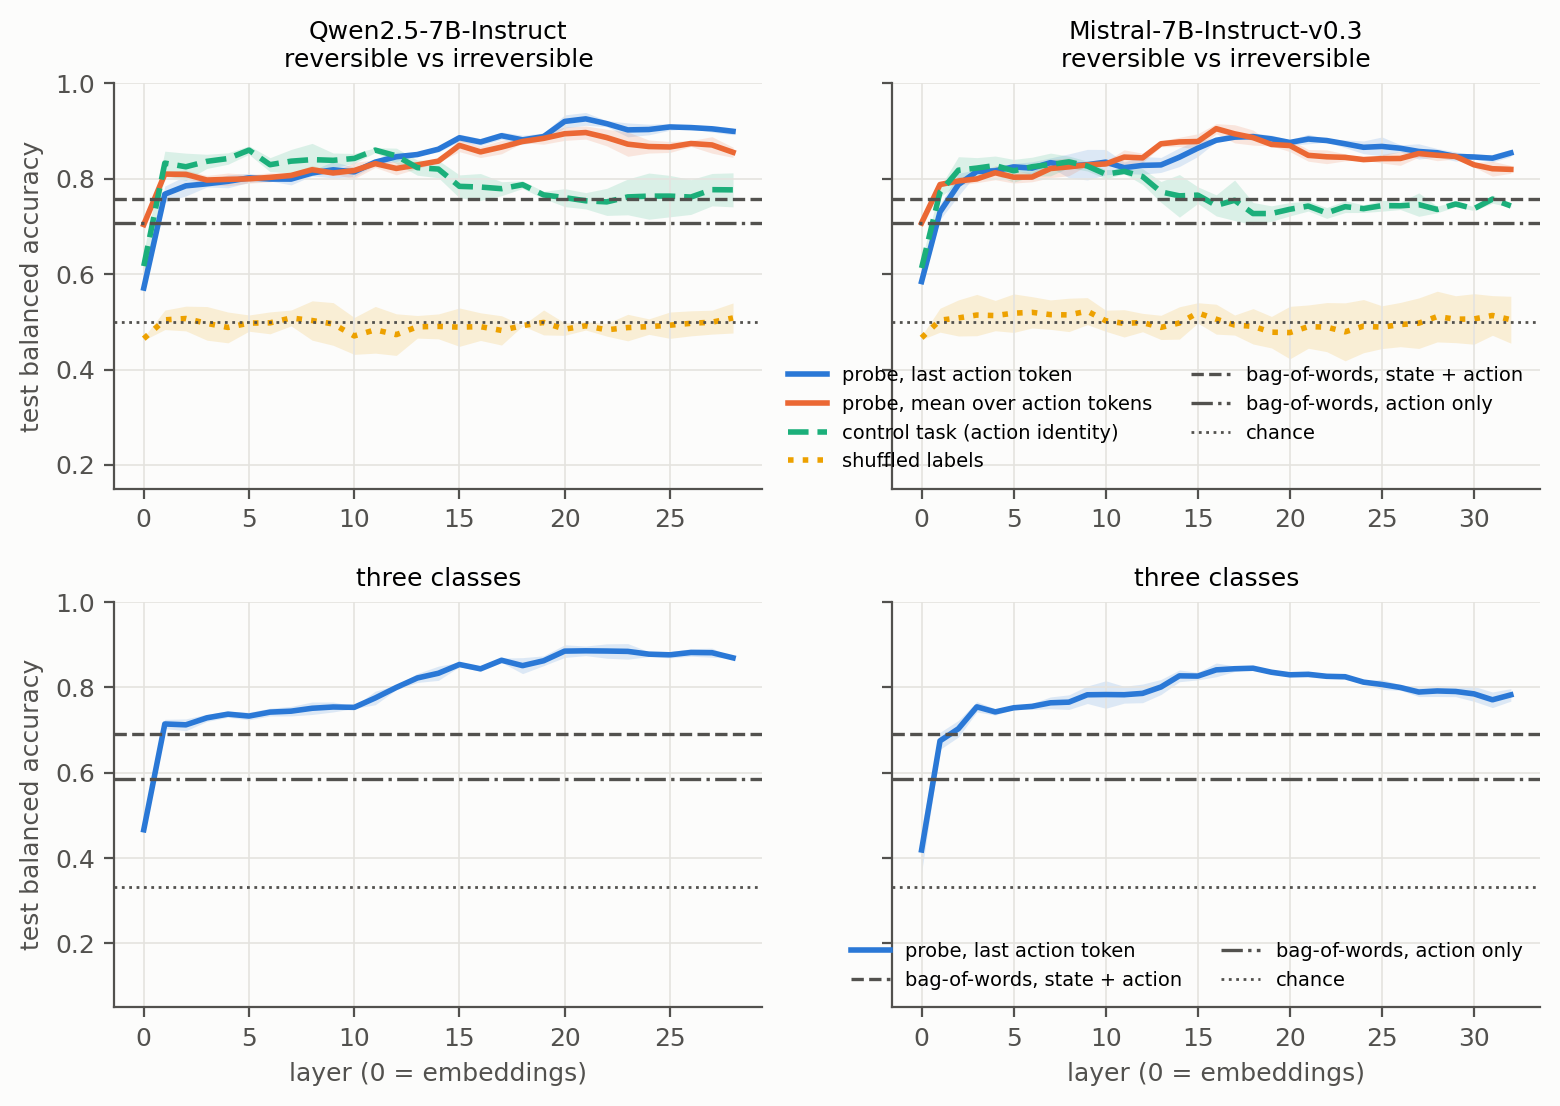
\includegraphics[width=0.9\textwidth]{probe_layers.png}
\caption{Test balanced accuracy of linear probes by layer (mean over three splits, band = one
standard deviation), with the shuffled-label probe, the action-identity control task, the two
bag-of-words baselines and chance.}
\label{fig:layers}
\end{figure*}

\begin{table}[t]
\centering
\small
\begin{tabular}{lcc}
\toprule
 & Qwen (L20) & Mistral (L17) \\
\midrule
Binary probe, all test ($n{=}383$) & .920 {\scriptsize[.870, .931]} & .887 {\scriptsize[.853, .917]} \\
\quad macro-F1 / AUROC & .921 / .970 & .888 / .949 \\
\quad minimal pairs ($n{=}192$) & .910 {\scriptsize[.849, .938]} & .849 {\scriptsize[.801, .904]} \\
\quad ScienceWorld ($n{=}95$) & .847 {\scriptsize[.688, .866]} & .841 {\scriptsize[.725, .900]} \\
Three-class probe ($n{=}527$) & .885 {\scriptsize[.845, .901]} & .844 {\scriptsize[.802, .867]} \\
\midrule
Majority class & .500 & .500 \\
BoW, action only & .708 & .708 \\
\quad minimal pairs & .500 & .500 \\
BoW, state + action & .757 & .757 \\
\quad minimal pairs & .710 & .710 \\
Layer 0 (embeddings) & .571 & .584 \\
Shuffled labels & .485 & .493 \\
Control task, verb & .995 & .991 \\
Control task, action identity & .760 & .755 \\
\midrule
Selectivity, verb & $-.075$ & $-.104$ \\
Selectivity, action identity & $+.160$ & $+.132$ \\
\bottomrule
\end{tabular}
\caption{RQ1. Balanced accuracy at the best layer (chosen by training cross-validation). Values
are means over three splits; brackets are 95\% bootstrap intervals for the first split. Baselines
and controls are for the binary task.}
\label{tab:rq1}
\end{table}

Figure~\ref{fig:layers} and Table~\ref{tab:rq1} give the main result. A linear probe separates
reversible from irreversible actions with balanced accuracy 0.920 on Qwen (layer 20 of 28) and
0.887 on Mistral (layer 17 of 32). Accuracy rises from near chance at the embedding layer
(0.571 and 0.584), passes the bag-of-words baselines in the first few layers and peaks in the
upper-middle of the network.

The minimal pairs are the informative test. The action text is identical within a triple, so the
action-only baseline is exactly at chance (0.500). The stronger bag-of-words baseline on state
plus action reaches 0.710, because all policy lines are visible and irreversible-sounding words
are weakly correlated with the label. The probe reaches 0.910 (Qwen) and 0.849 (Mistral) on the
same items. The probe is therefore not only detecting words such as ``delete''.

\paragraph{Controls.} Shuffled labels give chance. The control task with one random label per
verb is solved almost perfectly (0.995, 0.991), so selectivity against it is negative. This is
expected: there are few verbs, verb identity is trivially decodable, and the control labels of
test items are determined by their verbs. That control is uninformative here. With a random
label per action identity the probe must memorise several hundred types; control accuracy falls
with depth while task accuracy rises (Figure~\ref{fig:layers}), giving selectivity of $+0.160$
and $+0.132$ at the best layer.

\begin{table}[t]
\centering
\small
\begin{tabular}{lcc}
\toprule
Ablation (binary unless stated) & Qwen & Mistral \\
\midrule
Last action token (main) & .920 & .887 \\
Mean over action tokens & .895 & .905 \\
Trained and tested on minimal pairs & .906 & .873 \\
Three classes & .885 & .844 \\
\midrule
Train sandbox $\to$ test ScienceWorld & .510 & .571 \\
Train ScienceWorld $\to$ test sandbox & .500 & .500 \\
\midrule
ScienceWorld labels, horizon 1 & .856 & .835 \\
ScienceWorld labels, horizon 2 & .884 & .873 \\
ScienceWorld labels, horizon 3 & .881 & .863 \\
\midrule
Held out: \texttt{delete\_file} & .504 (.852) & .625 (.691) \\
Held out: \texttt{edit\_file} & .613 (.802) & .662 (.711) \\
Held out: \texttt{send\_email} & .654 (.919) & .517 (.848) \\
Held out: \texttt{transfer\_money} & .725 (.884) & .671 (.769) \\
\bottomrule
\end{tabular}
\caption{Ablations at the best layer (balanced accuracy; AUROC in parentheses for the held-out
tool-family experiment). Horizon rows use ScienceWorld items only ($n{=}95$ test items).}
\label{tab:ablations}
\end{table}

\paragraph{Ablations (Table~\ref{tab:ablations}).} Token position matters little. Training and
testing on minimal pairs alone gives 0.906 and 0.873. The label horizon (1, 2 or 3 steps)
changes ScienceWorld accuracy by less than its split-to-split variation.

Two ablations limit what the probe result means. First, probes do not transfer between
environments: trained on the sandbox and tested on ScienceWorld they score 0.510 and 0.571, and
the reverse direction is at chance. Second, a probe trained on three sandbox tool families and
tested on the fourth reaches only 0.50 to 0.73 balanced accuracy. On Qwen the AUROC in that
experiment stays between 0.80 and 0.92, so the learned direction still ranks the held-out
family's items in the right order while the decision threshold is wrong; on Mistral the AUROC is
lower (0.69 to 0.85). What is linearly decodable is thus largely specific to a tool and its
policy. We do not find one environment-independent ``irreversible'' direction.

\subsection{RQ2: stated answers are poor and disagree with the probe}

\begin{table}[t]
\centering
\small
\begin{tabular}{lcc}
\toprule
 & Qwen & Mistral \\
\midrule
Stated accuracy, all ($n{=}2710$) & .397 {\scriptsize[.380, .416]} & .421 {\scriptsize[.401, .440]} \\
\quad sandbox ($n{=}2160$) & .440 & .379 \\
\quad ScienceWorld ($n{=}550$) & .231 & .585 \\
\quad minimal pairs ($n{=}1440$) & .433 & .361 \\
Probe accuracy, all (out-of-fold) & .895 {\scriptsize[.883, .906]} & .856 {\scriptsize[.843, .868]} \\
\quad minimal pairs & .857 & .789 \\
\midrule
$\kappa$ stated vs.\ probe & .147 & .062 \\
$\kappa$ stated vs.\ true label & .154 & .058 \\
$\kappa$ probe vs.\ true label & .841 & .781 \\
\midrule
Probe right, stated wrong & 53.2\% & 48.0\% \\
Stated right, probe wrong & 3.4\% & 4.5\% \\
Most frequent stated answer & PARTIAL 77\% & REVERSIBLE 95\% \\
\bottomrule
\end{tabular}
\caption{RQ2. Three-way accuracy of the stated answer and of the three-class probe (out-of-fold,
best layer), and Cohen's $\kappa$. No answer was unparseable.}
\label{tab:rq2}
\end{table}

Asked directly, both models answer badly (Table~\ref{tab:rq2}). Qwen answers PARTIAL for 77\% of
pairs and Mistral answers REVERSIBLE for 95\%; three-way accuracy is 0.397 and 0.421, where
always giving the most frequent true label would score 0.387. Agreement between the stated
answer and the true label is slight ($\kappa = 0.154$ and $0.058$), and so is agreement between
the stated answer and the probe ($0.147$ and $0.062$), while the probe agrees well with the true
label ($0.841$ and $0.781$). In about half of all pairs the probe is right and the stated answer
is wrong. What the model says does not match what its hidden state encodes.

\subsection{RQ3: agents do not act on reversibility}

\begin{table*}[t]
\centering
\small
\begin{tabular}{llccccccc}
\toprule
Model & Prompt & Irrev.\ action & Caution & Over-caution & Sensitivity & McNemar & Success & Parse \\
 & & rate & (irrev.) & (rev.) & & $p$ & irr.\ / rev. & fail \\
\midrule
Qwen & neutral & .950 {\scriptsize[.883, 1.00]} & .217 {\scriptsize[.116, .333]} & .200 {\scriptsize[.100, .317]} & $+.017$ {\scriptsize[.000, .050]} & 1.00 & .983 / .917 & .000 \\
Qwen & careful & .983 {\scriptsize[.950, 1.00]} & .200 {\scriptsize[.100, .317]} & .233 {\scriptsize[.133, .350]} & $-.033$ {\scriptsize[$-$.083, .000]} & 0.50 & 1.00 / .950 & .002 \\
Mistral & neutral & .950 {\scriptsize[.883, 1.00]} & .083 {\scriptsize[.017, .167]} & .100 {\scriptsize[.033, .183]} & $-.017$ {\scriptsize[$-$.050, .000]} & 1.00 & .933 / .933 & .026 \\
\bottomrule
\end{tabular}
\caption{RQ3 on 60 task pairs (120 runs per row). Brackets are 95\% bootstrap intervals over
pairs. Sensitivity is caution rate on the irreversible version minus caution rate on the
reversible version.}
\label{tab:rq3}
\end{table*}

\begin{figure}[t]
\centering
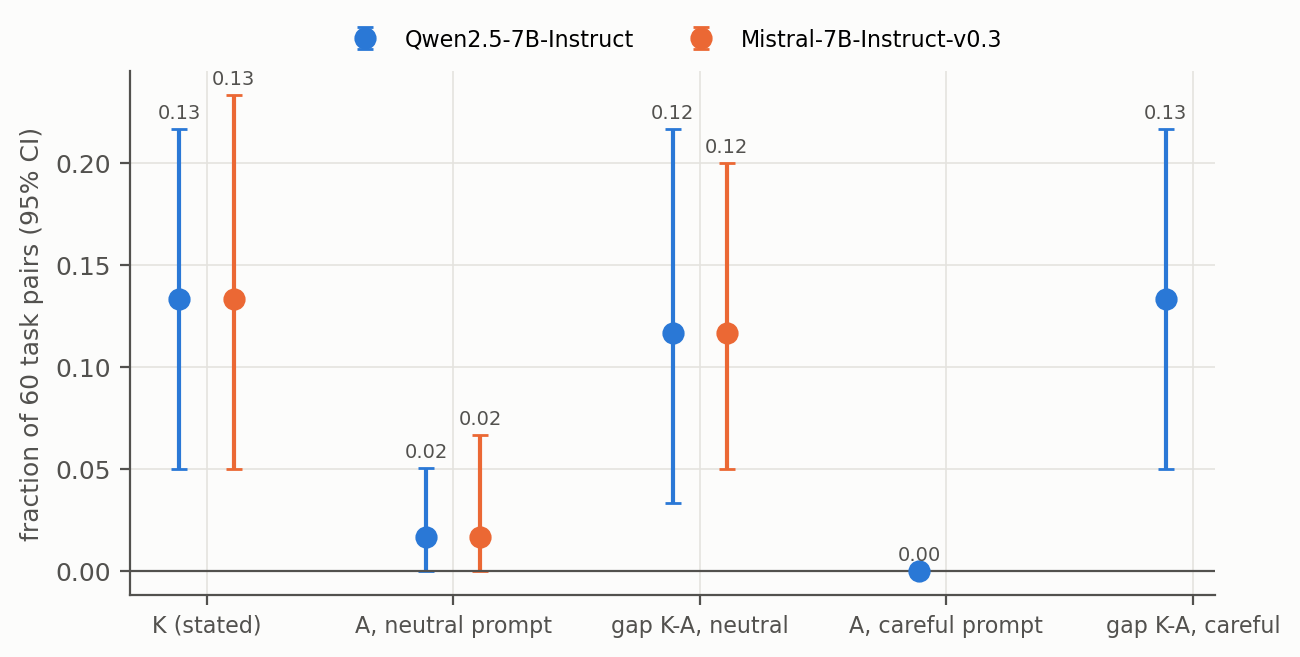
\includegraphics[width=\columnwidth]{blindness_gap.png}
\caption{$K$, $A$ and the blindness gap $K-A$ with 95\% bootstrap intervals over 60 task pairs.
The careful-prompt condition was run for Qwen only.}
\label{fig:gap}
\end{figure}

\begin{figure}[t]
\centering
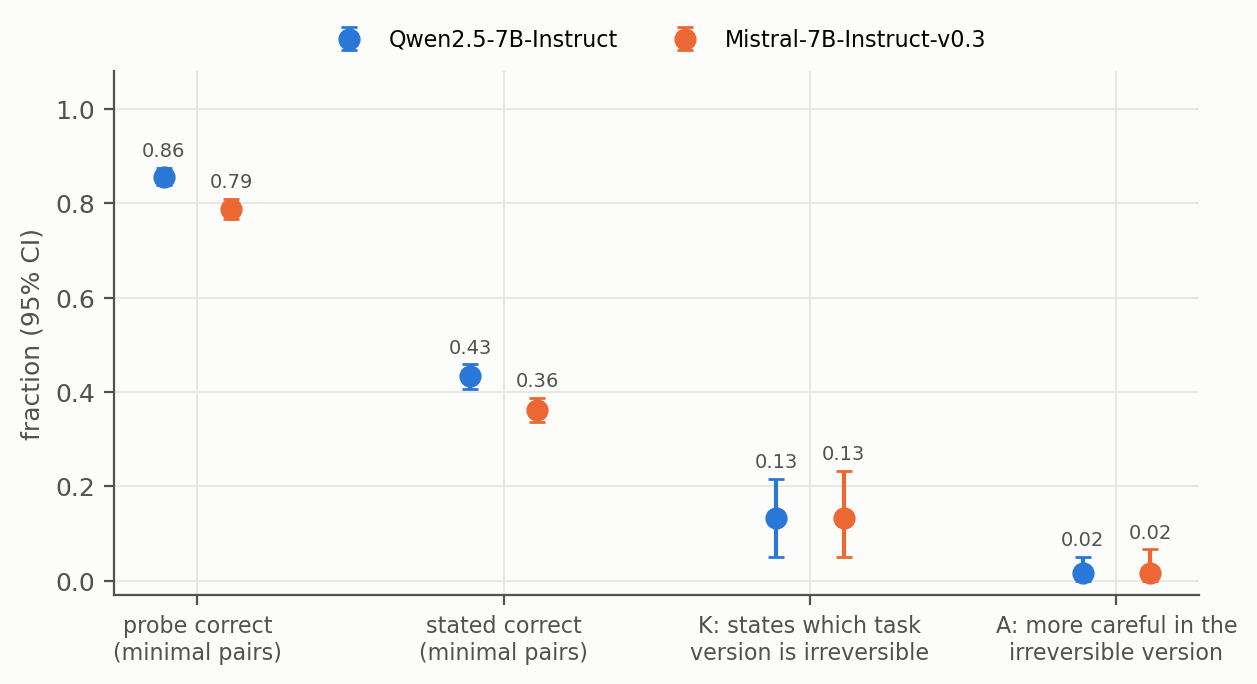
\includegraphics[width=\columnwidth]{stated_probe_behaviour.png}
\caption{Probed, stated and behavioural measures side by side. The first two are on the 1,440
minimal-pair items of the dataset; $K$ and $A$ are on the 60 task pairs.}
\label{fig:compare}
\end{figure}

Both agents take the irreversible action in 95\% of the irreversible task versions
(Table~\ref{tab:rq3}), and almost equally often in the reversible versions (0.967 and 0.950).
Caution before the risky call is rare and does not depend on reversibility: sensitivity is
$+0.017$ for Qwen and $-0.017$ for Mistral, with McNemar $p = 1.0$ in both. Under the strict
definition of caution, sensitivity is exactly 0 for both models.

Qwen's caution comes almost entirely from one family. In 10 of 15 transfer tasks it reads the
invoice before paying, and usually also asks the user, in both versions alike. This looks like a
response to the invoice text rather than to the settlement policy. Before its first risky call it
never makes a backup and never chooses the safer tool. Mistral never asks the user before its
first risky call.

\paragraph{System-prompt ablation.} Adding ``Some actions cannot be undone. Before any
irreversible action, check the current state, and confirm with the user or use a safer
alternative'' to Qwen's system prompt does not help: the irreversible action rate is 0.983 and
sensitivity is $-0.033$. A simple instruction does not close the gap.
The careful-prompt condition was not run for Mistral.

\paragraph{Blindness gap.} $K$ is 0.133 for both models: each states IRREVERSIBLE for the
irreversible version and REVERSIBLE for the reversible one in 8 of 60 pairs. $A$ is 0.017 for
both: the agent is more careful in the irreversible version in 1 of 60 pairs. The gap $K - A$
(Figure~\ref{fig:gap}) is 0.117 (Qwen, 95\% interval [0.033, 0.217]; Mistral, [0.050, 0.200]). It is positive but small,
and it is small because $K$ is low, not because $A$ is high. With the lenient
$K_{\mathrm{ord}}$ (added after a smoke test, see Section~3.6) the gap is 0.433
[0.300, 0.567] for Qwen and 0.117 [0.050, 0.200] for Mistral.

The larger disconnect is upstream of the stated answer (Figure~\ref{fig:compare}). On the
dataset's minimal pairs the probe is right for 86\% (Qwen) and 79\% (Mistral) of items, the
stated answer for 43\% and 36\%, and behaviour distinguishes the two versions of a task in 2\%
of pairs. These measures are on different item sets and are not directly subtractable, but the
ordering is the same in both models: decodable, mostly not stated, and not acted on.

\subsection{RQ4: steering changes behaviour, but not towards caution}

\begin{figure*}[t]
\centering
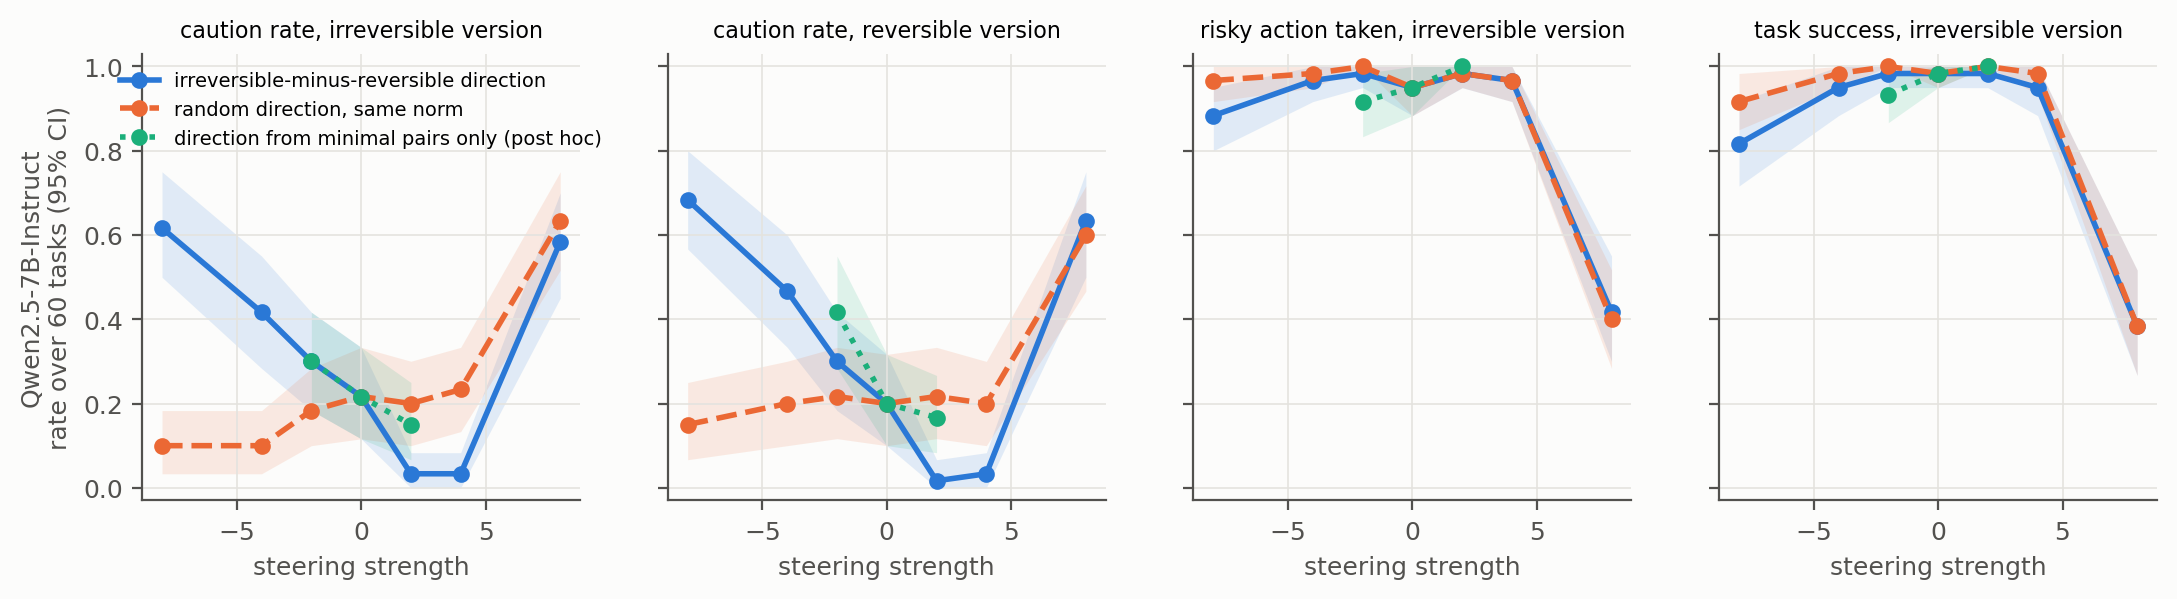
\includegraphics[width=\textwidth]{steering_curve.png}
\caption{Steering Qwen at layer 20 during the agent runs. Bands are 95\% bootstrap intervals over
60 tasks. Strength 0 is the unsteered run. The dotted line is the post-hoc control direction
computed from minimal pairs only, which was run at $\pm 2$.}
\label{fig:steer}
\end{figure*}

\begin{table*}[t]
\centering
\small
\begin{tabular}{r|cccccc|cccccc}
\toprule
 & \multicolumn{6}{c|}{Irreversible-minus-reversible direction} & \multicolumn{6}{c}{Random direction, same norm} \\
$\alpha$ & Caut.\ irr. & Caut.\ rev. & Inspect & Risky & Success & Parse fail & Caut.\ irr. & Caut.\ rev. & Inspect & Risky & Success & Parse fail \\
\midrule
$-8$ & .617 & .683 & .600 & .883 & .817 & .150 & .100 & .150 & .100 & .967 & .917 & .177 \\
$-4$ & .417 & .467 & .400 & .967 & .950 & .040 & .100 & .200 & .100 & .983 & .983 & .003 \\
$-2$ & .300 & .300 & .283 & .983 & .983 & .031 & .183 & .217 & .183 & 1.00 & 1.00 & .003 \\
0 & .217 & .200 & .167 & .950 & .983 & .000 & .217 & .200 & .167 & .950 & .983 & .000 \\
$+2$ & .033 & .017 & .033 & .983 & .983 & .000 & .200 & .217 & .183 & .983 & 1.00 & .000 \\
$+4$ & .033 & .033 & .033 & .967 & .950 & .003 & .233 & .200 & .200 & .967 & .983 & .000 \\
$+8$ & .583 & .633 & .000 & .417 & .383 & .406 & .633 & .600 & .050 & .400 & .383 & .471 \\
\bottomrule
\end{tabular}
\caption{RQ4 on Qwen (60 task pairs per row and direction). Caut.: caution rate on the
irreversible and reversible versions. Inspect, Risky and Success are for the irreversible
version: state inspected before the risky call, risky call made, task completed. Parse fail is
the fraction of steps without a valid tool call.}
\label{tab:steer}
\end{table*}

The direction at layer 20 of Qwen has norm 8.7; the mean hidden-state norm at that position is
86.2, so strengths 2, 4 and 8 add about 20\%, 40\% and 81\% of a typical state.

Steering along the direction has a clear, graded effect that the random direction does not have
(Figure~\ref{fig:steer}, Table~\ref{tab:steer}), but the effect is the reverse of the hypothesis.
Pushing \emph{towards} ``irreversible'' ($\alpha = +2, +4$) reduces the caution rate on
irreversible tasks from 0.217 to 0.033. Pushing \emph{away} from it raises the rate to 0.300,
0.417 and 0.617 at $\alpha = -2, -4, -8$. With the random direction the rate stays between 0.100
and 0.233 over the same range. The change is carried by state inspection (reading a file before
acting), which moves from 0.600 at $\alpha=-8$ to 0.033 at $\alpha=+4$; asking the user becomes
rarer under any perturbation, including the random one.

Three further observations qualify this. (i) The agent still makes the risky call: the
irreversible action rate stays at or above 0.88 for every strength up to $|\alpha| = 4$ and for
$\alpha=-8$, so steering changes what happens before the action, not whether it happens.
(ii) Steering never makes the agent more careful in the irreversible version than in the
reversible one. Caution moves about equally in both versions, and sensitivity stays within $\pm 0.07$ of zero for the
probe direction (McNemar $p \geq 0.25$ at every strength). The one nominally significant value among
the 12 steered conditions is the random direction at $\alpha=-4$ ($-0.100$, $p = 0.03$, uncorrected).
(iii) $\alpha = +8$ is over-steering for both directions. Task success falls to 0.383, about
40\% of steps are not valid tool calls, and the apparent rise in caution (0.583 and 0.633) is
the agent failing to act, not the agent being careful.

We therefore find no evidence that the linearly decodable reversibility signal drives careful
behaviour. One candidate explanation for the reversed effect is that a difference of class means
is not a pure reversibility direction. Read-only tools are all in the reversible class, so the
direction also separates ``reading'' from ``acting'', and moving towards the reversible side
could simply make the agent read more.

\paragraph{Post-hoc control: a direction from minimal pairs.} To test this explanation we
computed the same difference of means on minimal-triple training items only, where the action
text is identical across classes and tool identity cancels. This direction has a third of the
norm of the main one (2.8 against 8.7) and cosine similarity 0.38 with it, so most of the main
direction is indeed not about reversibility. We rescaled it to the norm of the main direction
and steered at $\alpha = \pm 2$. This control was added after seeing the main result, and the
runs at $\pm 4$ did not complete because the cluster's shared quota was exhausted. At
$\alpha=-2$ the caution rate is 0.300 on irreversible tasks and 0.417 on reversible ones; at
$\alpha=+2$ it is 0.150 and 0.167 (unsteered: 0.217 and 0.200). The sign is the same as for the
main direction and the effect is weaker. Removing tool identity therefore does not turn the
direction into one that produces caution, and the read-versus-act confound is not the whole
explanation. At $\alpha=-2$ caution was higher in the \emph{reversible} version (sensitivity
$-0.117$, McNemar $p = 0.016$, uncorrected), which is the opposite of the dependence one would
want.

\section{Limitations}

\begin{itemize}
\item \textbf{Small sandbox.} Four policy-governed tool families and ten fixed tools. The probe
may be learning twelve tool--policy conjunctions; the held-out-family and cross-environment
results suggest that it largely is.
\item \textbf{ScienceWorld labels.} The search is exhaustive only at depth 1 and uses a beam at
depths 2 and 3, the state signature covers only the current room and the inventory, there is no
partial class, and 124 of the 220 irreversible pairs use the verb \emph{eat}. The ScienceWorld
test split has 95 items, so its intervals are wide.
\item \textbf{Human agreement is missing.} The two-annotator check on 100 pairs has not been
done yet, so there is no $\kappa$ between annotators or against the automatic labels.
\item \textbf{Models.} Two 7B models. The second family is Mistral, not the Llama-3.1-8B named
in the brief. The 14B size ablation was not run.
\item \textbf{One wording per measurement.} The stated-answer question and the task texts each
have one fixed wording. Both models show a strong answer bias (PARTIAL, REVERSIBLE), and a
different question format could change stated accuracy and $K$.
\item \textbf{Task design.} The user explicitly suggests the quick route, and \texttt{ask\_user}
always approves. Mistral rarely calls \texttt{done} and repeats calls (13.2 steps on average),
so its trajectories are noisy after the first action. In the reversible email tasks Qwen
sometimes unsends and resends repeatedly, which lowers success there.
\item \textbf{Protocol change.} Stopping generation at the end of the tool call was added after
Qwen's unsteered runs; 1 of 771 steps in those runs had text outside the JSON object.
\item \textbf{Layer selection.} The best layer is chosen by cross-validation on the training
portion of the first split and reused for the other two splits, whose test items overlap that
training portion.
\item \textbf{Steering.} One model and one layer, with the direction added at all positions.
The minimal-pair control direction was added post hoc and ran at $\pm 2$ only.
\item \textbf{System-prompt ablation.} Run for Qwen only.
\item \textbf{Horizon.} Labels use a 3-step horizon.
\item \textbf{Not done.} RQ5 (uncertainty), the ToolEmu cases and Mistral steering.
\end{itemize}

\section{Conclusion}

In both models reversibility can be read from hidden states with a linear probe, including
on minimal pairs that defeat lexical baselines. That signal is not reflected in what the models
say (about 40\% accuracy, $\kappa \leq 0.15$ with the probe) or in what the agents do (95\%
irreversible action rate, sensitivity indistinguishable from zero). The blindness gap as defined
from stated answers is small ($K - A = 0.12$) only because the stated answers are themselves
poor. Steering shows that the probe direction matters causally for behaviour, but pushing towards
``irreversible'' made the agent inspect less, not more, and no strength made it more careful in
the irreversible version of a task than in the reversible one. The decodable signal also does not generalise across tool
families or environments. The most direct next steps are to complete the
minimal-pair steering control at larger strengths and other layers, to compute a probe-based
version of $K$ on the task prompts themselves, and to repeat the measurements on larger models.

\bibliography{refs}

\end{document}
